\documentclass[a4paper]{article}
\usepackage{amsmath}
\usepackage{graphicx}
\usepackage[margin=1in]{geometry}
\usepackage{setspace}
\usepackage{subfigure}
\usepackage{multirow}
\usepackage{caption}
\usepackage[table]{xcolor}
\linespread{1.2}

\usepackage{listings}
\begin{document}
    \title{Math 128A Programming Assignment 3}
    \author{\textsc{YIMO ZHU}}
    \date{\today}
    \maketitle
    %���ɱ���
\section{Question \#1}
In this question we will write a a function to output the unit Legendre Polynomials' evaluation, which each of them has a unit inner product with itself, over the designated m points. Under each designated point x, the way to recover the evaluations of polynomials up to degree n can be done by the following recursive system:
\[
\sqrt{b_{1}}\phi_{1}(x) = (x-a_0)\phi_0(x)\]
\[
\sqrt{b_{n+1}}\phi_{n+1}(x) = (x-a_n)\phi_n(x) - \sqrt{b_n}\phi_{n-1}(x)
\]
Where the coefficients $\{a_n\}$ and $\{b_n\}$ are usually specified at $a_n = 0$ and $b_n = \frac{n^2}{4n^2-1}$.\\
What I did in the program is to first check the input a and b. Their length has to differ by exactly one. After doing that, first we generate the output matrix, with size $(n+1,m)$, we temporarily use 0 to fill all the positions.\\
Then we start the main loop, in each loop we fix the evaluation point. And generate a one dimensional vector to store the polynomials' evaluation at this specific point. Then we use the recursive system to fill all the position in the one dimensional vector. After this is done, we put the one dimensional vector into the proper place in the output matrix.\\
Hence, by iterating through all of the evaluation points, we can construct the output matrix PHI. \\
The two graph, which visualizing $\phi_{10}$ and $\phi_{50}$ over the interval $[-1,1]$, are included below.
\begin{figure}[!ht]
  \centering
  % Requires \usepackage{graphicx}
  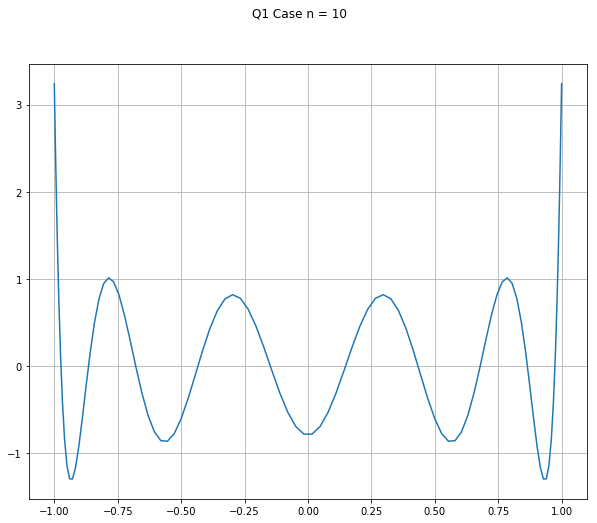
\includegraphics[scale=0.5]{Q1Case10.png}
\end{figure}
\begin{figure}[!ht]
  \centering
  % Requires \usepackage{graphicx}
  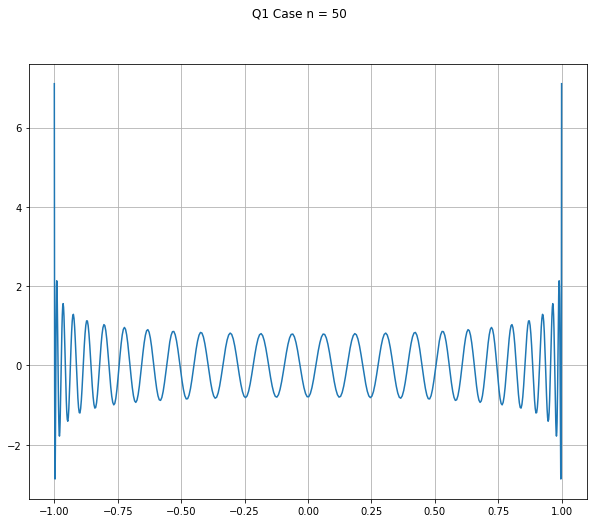
\includegraphics[scale=0.5]{Q1Case50.png}\\
\end{figure}
\section{Question \#2}
To achieve the same goal as in the question number 1, we have an alternative method. It can be shown that the recursive system also gives the coefficients of the polynomials up to degree n. So in this sense, we first get all of the coefficients, then evaluate the polynomial using a nested algorithm.\\
To do this job, we first construct a all zero n+1 by n+1 matrix. Then, iterate through all of the degree up to n. At each stage, a multiplier $x$ will increase the former polynomial by exactly 1 degree.\\
The plot generated using this method are included below:
\begin{figure}[!ht]
  \centering
  % Requires \usepackage{graphicx}
  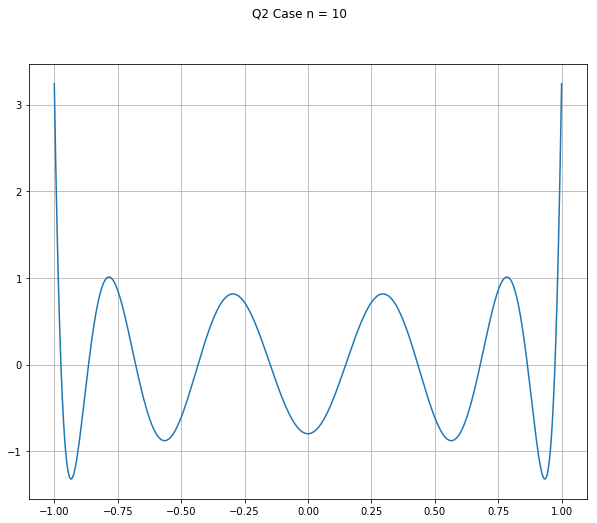
\includegraphics[scale=0.5]{Q2Case10.png}
\end{figure}
\begin{figure}[!ht]
  \centering
  % Requires \usepackage{graphicx}
  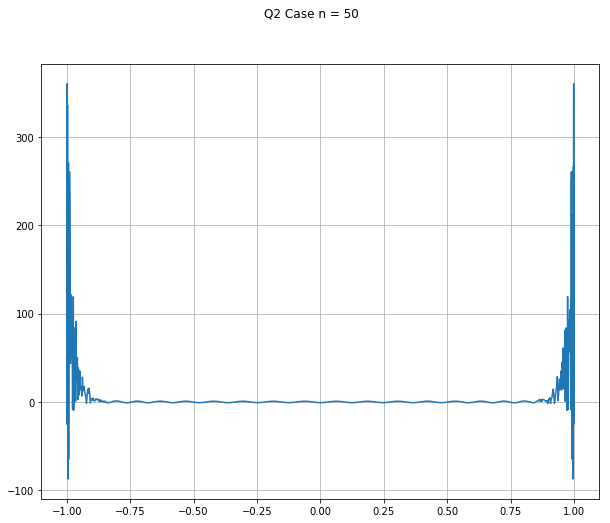
\includegraphics[scale=0.5]{Q2Case50.png}\\
\end{figure}
\section{Q1 \& Q2 comments}
The main presentation of the result of Q1 and Q2 can be seen from the 4 plots. We can see that the "good" method and the "bad method" are approximately the same when n is small, eg. $n = 10$. But when n gets large, which means that the volatility of the function gets larger and the degree gets higher, the round off error kicks in. That makes the "bad method" perform extremely bad at the endpoints of the interval. While the "good method" can still give a stable result.
\section{Question 3}
In this question, we will use the Golub-Welsch algorithm to get the Guassian quadrature's abscissas and weights. It's a easy work to do once we know how the algorithm works.\\
Firstly, we use a row by row iterative manner to form the coefficients matrix $A$. Then, we use the linear algebra function of Numpy to get the eigenvalue and the eigenvector of $A$. After doing that, we just need to slice out the target part of the eigenvector matrix to get the weight.\\
Then we use these abscissas and weights to implement Guassian quadrature. I did in n = 10 and 80.\\
\begin{center}
The weights and abscissas for n = 10 is below:
\\
\begin{tabular}{|l|l|l|}
\hline
 & abscissas & weight \\
\hline
0 & -0.9739065285171732 & 0.06667134430868969 \\
\hline
1 & -0.8650633666889858 & 0.14945134915058003 \\
\hline
2 & -0.6794095682990245 & 0.2190863625159812 \\
\hline
3 & -0.4333953941292474 & 0.26926671930999607 \\
\hline
4 & -0.14887433898163108 & 0.2955242247147524 \\
\hline
5 & 0.14887433898163135 & 0.29552422471475304 \\
\hline
6 & 0.9739065285171714 & 0.0666713443086871 \\
\hline
7 & 0.8650633666889844 & 0.14945134915058197 \\
\hline
8 & 0.6794095682990242 & 0.21908636251598126 \\
\hline
9 & 0.4333953941292472 & 0.26926671930999657 \\
\hline
\end{tabular}
\\
The error sequence for n = 10 is below:
\\
\begin{tabular}{|l|l|}
\hline
 & E \\
\hline
0 & 4.440892098500626e-16 \\
\hline
1 & 9.43689570931383e-16 \\
\hline
2 & 2.3314683517128287e-15 \\
\hline
3 & 5.384581669432009e-15 \\
\hline
4 & 3.247402347028583e-15 \\
\hline
5 & 4.829470157119431e-15 \\
\hline
6 & 1.8388068845354155e-15 \\
\hline
7 & 5.1209037010835345e-15 \\
\hline
8 & 2.248201624865942e-15 \\
\hline
9 & 1.0824674490095276e-15 \\
\hline
10 & 8.708311849403572e-16 \\
\hline
11 & 2.7755575615628914e-15 \\
\hline
12 & 3.0270924655795284e-15 \\
\hline
13 & 9.71445146547012e-17 \\
\hline
14 & 5.532033164890038e-15 \\
\hline
15 & 5.551115123125783e-16 \\
\hline
16 & 1.7486012637846216e-15 \\
\hline
17 & 1.4432899320127035e-15 \\
\hline
18 & 5.2475385148298415e-15 \\
\hline
19 & 1.3128387266192476e-14 \\
\hline
20 & 1.5338519033217612 \\
\hline
\end{tabular}
\end{center}
\textbf{At last, the Norm of the error for n = 40 case is 1.3081472028338235e-13.}
\section{Question 4}
To do the same job as in question number 3, we can adopt the coefficients of the Legendre polynomials obtained in question number 2. We can directly solve the distinct roots of the corresponding polynomials, and solve for the weight by normalizing the polynomials' inner product. This is done by taking the inverse of the diag elements of polynomial's evaluation matrix.
\begin{center}
Again, the weights and abscissas is included here:\\
\begin{tabular}{|l|l|l|}
\hline
 & abscissas & weight \\
\hline
0 & -0.9739065285171801 & 0.06667134430866754 \\
\hline
1 & -0.8650633666889846 & 0.149451349150579 \\
\hline
2 & -0.6794095682990223 & 0.21908636251598373 \\
\hline
3 & -0.43339539412924777 & 0.2692667193099962 \\
\hline
4 & -0.14887433898163097 & 0.29552422471475287 \\
\hline
5 & 0.14887433898163122 & 0.2955242247147528 \\
\hline
6 & 0.43339539412924727 & 0.2692667193099964 \\
\hline
7 & 0.6794095682990238 & 0.21908636251598257 \\
\hline
8 & 0.8650633666889803 & 0.1494513491505835 \\
\hline
9 & 0.9739065285171762 & 0.06667134430867731 \\
\hline
\end{tabular}
\\
The error sequence is below:\\
\begin{tabular}{|l|l|}
\hline
 & E \\
\hline
0 & 2.8199664825478976e-14 \\
\hline
1 & 1.1962653090336062e-14 \\
\hline
2 & 2.786659791809143e-14 \\
\hline
3 & 2.768618667658984e-15 \\
\hline
4 & 1.4405143744511406e-14 \\
\hline
5 & 7.778500066280003e-15 \\
\hline
6 & 2.0011770018868447e-14 \\
\hline
7 & 1.1531140625686831e-14 \\
\hline
8 & 4.686528942698942e-14 \\
\hline
9 & 1.1518563880486e-15 \\
\hline
10 & 4.9096143817095594e-14 \\
\hline
11 & 1.3183898417423734e-15 \\
\hline
12 & 5.1800577716143437e-14 \\
\hline
13 & 2.4355517602714372e-14 \\
\hline
14 & 2.3517646163817574e-14 \\
\hline
15 & 2.1871393585115584e-14 \\
\hline
16 & 2.7332303087490573e-14 \\
\hline
17 & 3.1433189384699745e-15 \\
\hline
18 & 4.951768162175796e-14 \\
\hline
19 & 2.648575803121389e-14 \\
\hline
20 & 1.5338519033217901 \\
\hline
\end{tabular}
\end{center}
\textbf{At last, the Norm of the error sequence for n = 40 case is 0.01931741618118232.}
\section{Q3 \& Q4 comments}
The main point of these two question is to compare the accuracy using the weights and abscissas obtained by different methods to implement Gaussian quadrature. Actually, here we see that the abscissas and weights and the error sequence are generally the same in position or magnitude when n is as small as $n = 10$. But things start to diverge when n get larger up to $n = 40$. We can see that the absolute error norm change from a extremely small number that is to the 13 digits after the floating point, to a large deviation to only 2 digits after the floating point. Again, this is generated by the round-off error. So the lesson we learn here is to avoid storing high degree polynomials by memorizing their coefficients. Try to develop some recursive system to generate high degree polynomial, rather than let them jump out in the air, which will be highly unstable.\\
Another point here is that we see that for the last row of the error sequence, the error will explode all of a sudden. The reason why this is happening is exactly how the Guassian quadrature work. It can approximate those function that can be approximated by polynomial up to degree $2n-1$ very perfectly. But once the shape of the function kind of mess up and cannot be approached by polynomial within that range, the error can get out of control.
\end{document}